\documentclass[tikz,border=10pt]{standalone}
\usepackage{tikz}
\usetikzlibrary{shapes,arrows,positioning,fit,backgrounds}

\begin{document}
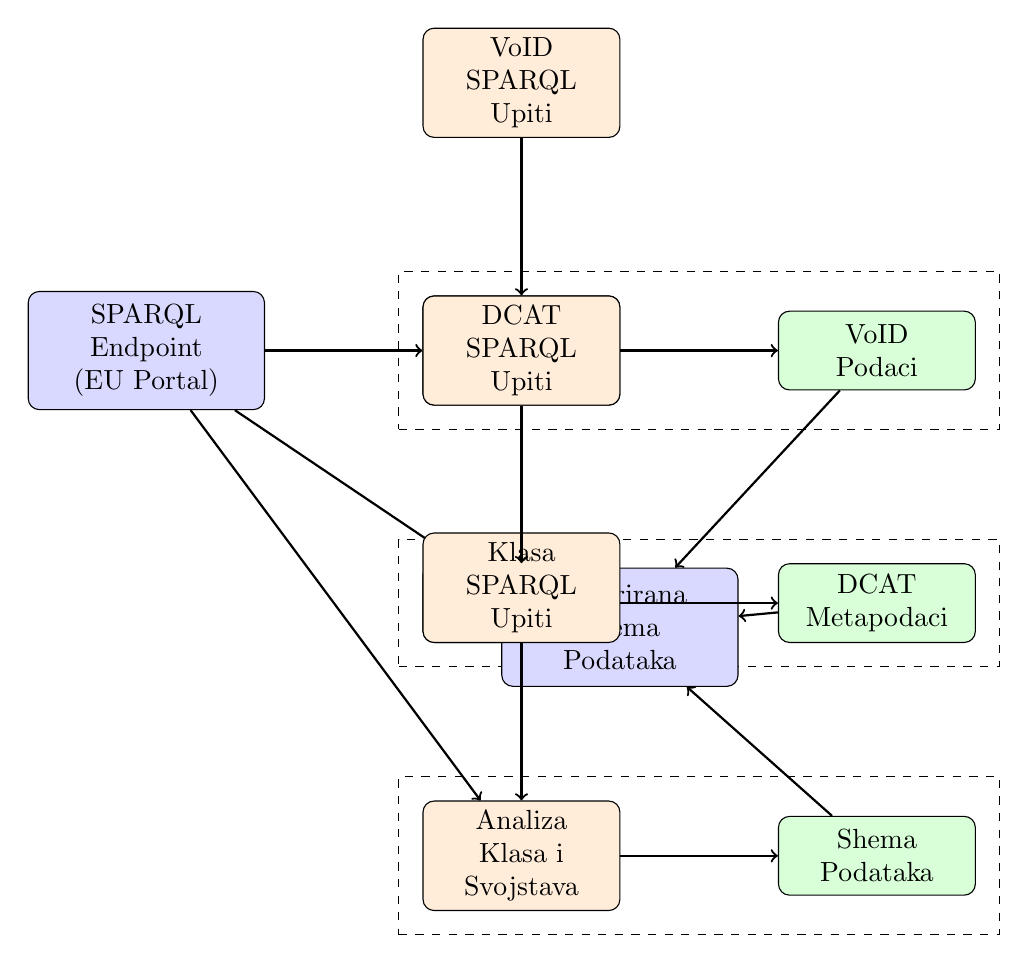
\begin{tikzpicture}[
    node distance=2cm,
    source/.style={rectangle, draw, rounded corners, minimum width=3cm, minimum height=1.5cm, align=center, fill=blue!15},
    process/.style={rectangle, draw, rounded corners, minimum width=2.5cm, minimum height=1cm, align=center, fill=orange!15},
    data/.style={rectangle, draw, rounded corners, minimum width=2.5cm, minimum height=1cm, align=center, fill=green!15},
    arrow/.style={->, thick},
    label/.style={font=\small}
]

% Data source
\node[source] (endpoint) {SPARQL\\Endpoint\\(EU Portal)};

% Extraction processes
\node[process, right=of endpoint] (void) {VoID\\Deskriptor\\Ekstrakcija};
\node[process, below=of void] (dcat) {DCAT\\Analiza};
\node[process, below=of dcat] (classes) {Analiza\\Klasa i\\Svojstava};

% Extracted data
\node[data, right=of void] (void_data) {VoID\\Podaci};
\node[data, right=of dcat] (dcat_data) {DCAT\\Metapodaci};
\node[data, right=of classes] (schema_data) {Shema\\Podataka};

% Schema integration
\node[source, below right=2cm and 3cm of endpoint] (integration) {Integrirana\\Shema\\Podataka};

% Background grouping
\begin{scope}[on background layer]
    \node[fit=(void)(void_data), draw, dashed, inner sep=0.3cm, label=above:VoID Analiza] {};
    \node[fit=(dcat)(dcat_data), draw, dashed, inner sep=0.3cm, label=above:DCAT Analiza] {};
    \node[fit=(classes)(schema_data), draw, dashed, inner sep=0.3cm, label=above:Strukturna Analiza] {};
\end{scope}

% Main flow arrows
\draw[arrow] (endpoint) -- (void);
\draw[arrow] (endpoint) -- (dcat);
\draw[arrow] (endpoint) -- (classes);

% Process to data
\draw[arrow] (void) -- (void_data);
\draw[arrow] (dcat) -- (dcat_data);
\draw[arrow] (classes) -- (schema_data);

% Integration arrows
\draw[arrow] (void_data) -- (integration);
\draw[arrow] (dcat_data) -- (integration);
\draw[arrow] (schema_data) -- (integration);

% SPARQL queries
\node[process, above=of void] (void_query) {VoID\\SPARQL\\Upiti};
\node[process, above=of dcat] (dcat_query) {DCAT\\SPARQL\\Upiti};
\node[process, above=of classes] (class_query) {Klasa\\SPARQL\\Upiti};

% Query connections
\draw[arrow] (void_query) -- (void);
\draw[arrow] (dcat_query) -- (dcat);
\draw[arrow] (class_query) -- (classes);

\end{tikzpicture}
\end{document} 